{\Large \bf tf2p2z}

{\it Transfer function between input and output: rational fraction with two poles and two zeros}

\begin{center}
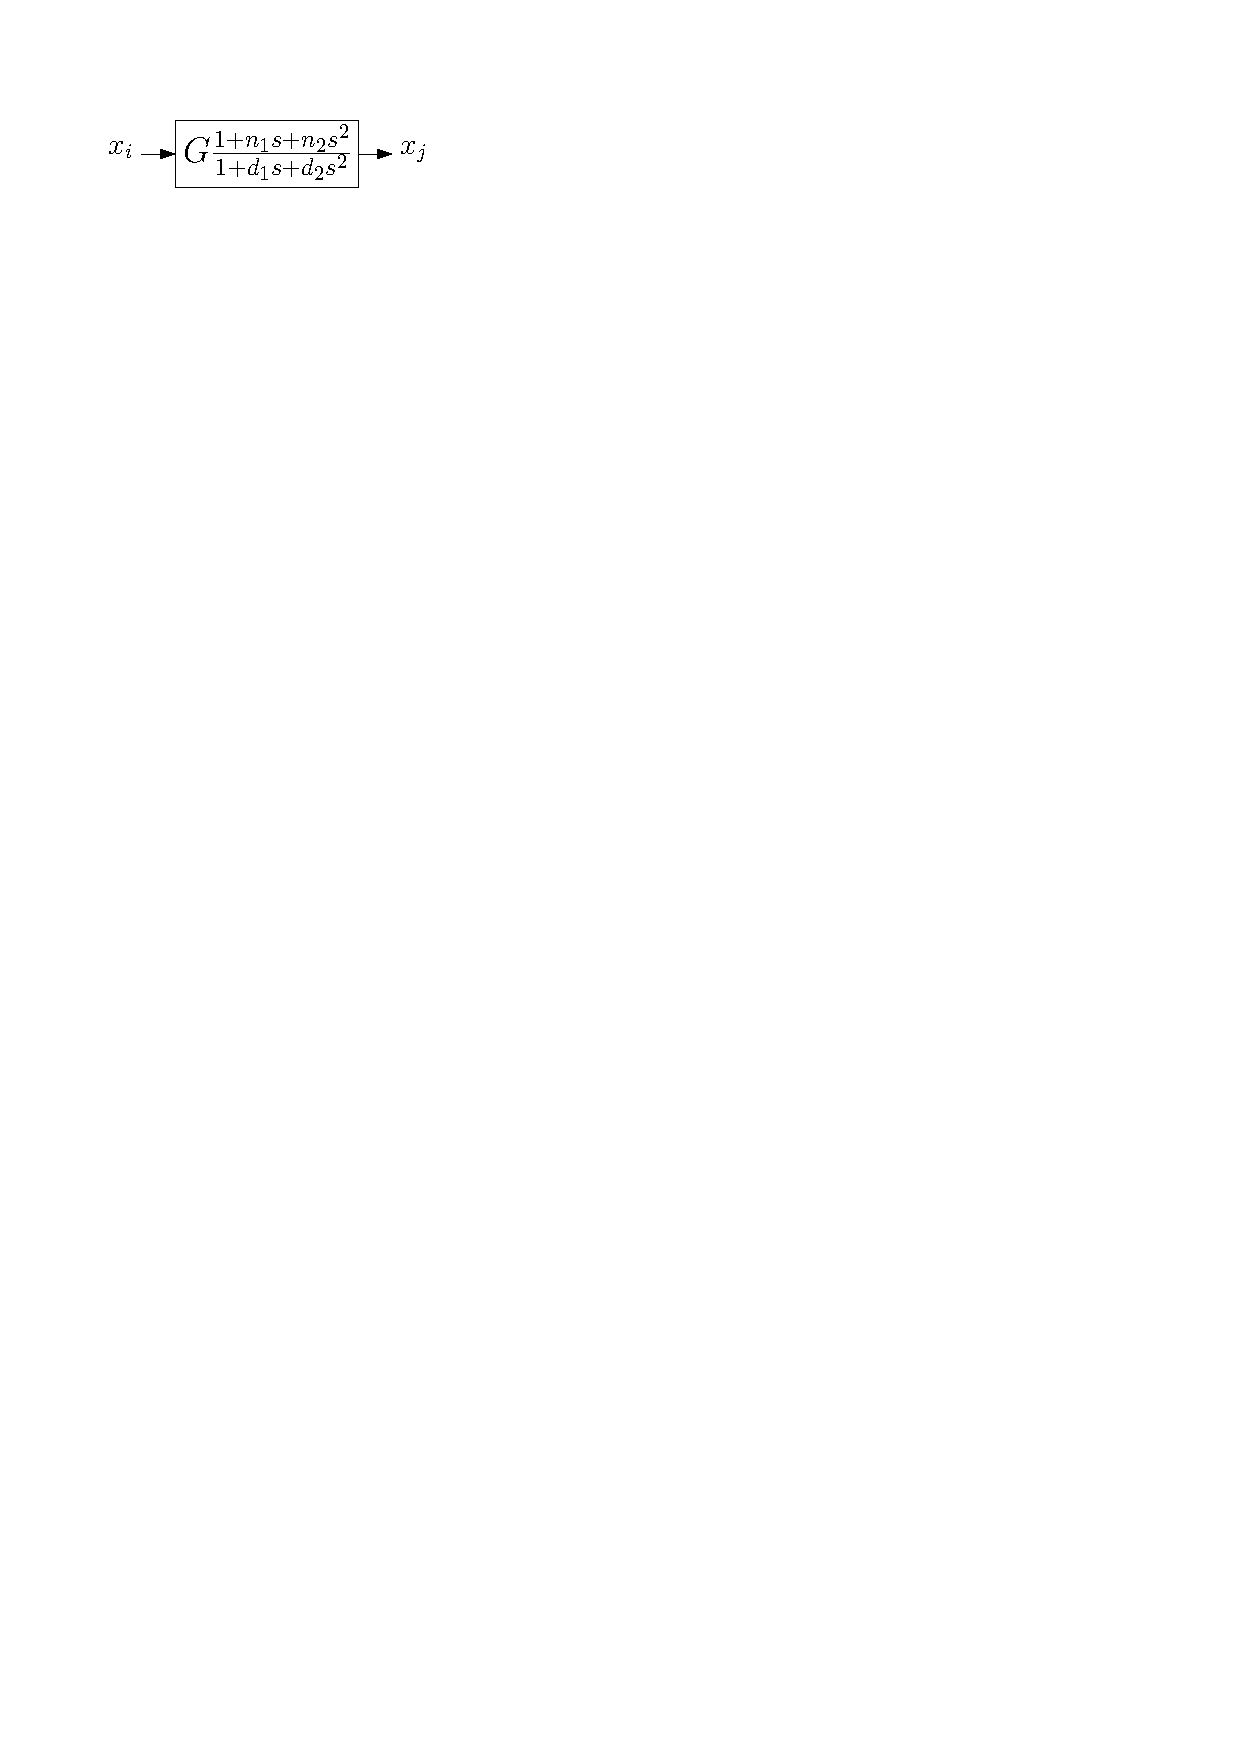
\includegraphics{tf2p2z.pdf}
\end{center}

Syntax : \hspace*{10ex}\parbox[t]{\textwidth}{\sf 
\& tf2p2z\\
name of variable $x_i$\\
name of variable $x_j$\\
data name, parameter name or math expression for $b_o$\\
data name, parameter name or math expression for $b_1$\\
data name, parameter name or math expression for $b_2$\\
data name, parameter name or math expression for $a_1$\\
data name, parameter name or math expression for $a_2$
}

~ \hrule ~

Internal states : $x_1$ ~~ and ~~ $x_2$

Discrete variables : none

\setcounter{equation}{0}

Equations : correspond to a second-order state space model with controllable canonical form:
\begin{eqnarray}
\dot{x_1} & = & x_2 \label{tf2p2z-1} \\
\dot{x_2} & = & - a_2 x_1 - a_1 x_2 + x_i \label{tf2p2z-2} \\
0 & = & (b_2 - a_2 b_o) x_1 + (b_1 - a_1 b_o) x_2 + b_o x_i - x_j \label{tf2p2z-3}
\end{eqnarray}

Initialization of internal states :

\begin{tabbing}
\hspace*{5ex} $x_2=0$ \\
\hspace*{5ex} if $a_2 \ne 0$ \= then $\displaystyle x_1 = \frac{x_i}{a_2}$ \\
\> else \= if $b_2 \ne 0$ \= then $\displaystyle x_1 = \frac{x_j}{b_2}$ \\
\> \> else $x_1 = 0$.
\end{tabbing}
\begin{itemize}
\item If $a_2$ is zero, the input state $x_i$ must be initially equal to zero in order the system to be in steady state. The value of $x_1$ is then obtained from (\ref{tf2p2z-3}) where $a_2=0$, $x_i=0$ and $x_2=0$.
\item If both $a_2$ and $b_2$ are zero, the transfer function has one pole and one zero only. Equations (\ref{tf2p2z-2}, \ref{tf2p2z-3}) do not involve $x_1$ any longer. Equation (\ref{tf2p2z-1}) becomes useless and $x_1$ is initialized to zero arbitrarily.
\end{itemize}

\vspace{2ex}

